\documentclass[main.tex]{subfiles}

\begin{document}
	
	\section{Band structure}\label{sec:band_structure}
	\subsection{Theory}
	In a crystal, the potential must necessarily be periodic in the unit cell, otherwise the discrete translational symmetry is broken. As such the following equation holds for any lattice vector $ \V{R} $:
	\begin{equation}\label{eq:band_period_V}
		V(\V{r}+\V{R}) = V(\V{r})
	\end{equation}
	Due to this periodicity, the potential can also be expressed as a sum over reciprocal lattice vectors. To see this, we start with the potential operator:
	\begin{equation}
		\hat{V} = \infint V(\V{r}) \ket{\V{r}}\bra{\V{r}}\ud \V{r} 
	\end{equation}
	Inserting two continuous identities for $ \V{k} $ and $ \V{k}' $, which is the equivalent of taking the Fourier transform of the potential: 
	\begin{align}
		\hat{V} &= \infint V(\V{r}) \bb{\infint \ket{\V{k}} \bra{\V{k}} \ud \V{k}  } \ket{\V{r}}\bra{\V{r}} \bb{\infint \ket{\V{k}'} \bra{\V{k}'} \ud \V{k}' } \ud \V{r} , \\
		&= \infint \infint \infint V(\V{r}) \ket{\V{k}} \braket{\V{k} | \V{r}} \braket{\V{r} | \V{k}'} \bra{\V{k}}  \ud\V{k}'   \ud\V{k}   \ud\V{r} .
	\end{align}
	The two middle brakets are $ \braket{\V{k}| \V{r}}= \sqrt{L^3}\inverse e^{-i \V{k} \D \V{r}} $ and $ \braket{\V{r} | \V{k}'} = \sqrt{L^3}\inverse e^{i \V{k}' \D \V{r}} $,  where $ L^3 $ is the volume of the material and $ \sqrt{L^3}\inverse $ is the normalization factor. This then becomes
	\begin{align}
		\hat{V} &= \frac{1}{L^3} \infint \infint  \infint  V(\V{r}) e^{-i(\V{k}-\V{k}') \D \V{r}} \ket{\V{k}} \bra{\V{k}'} \ud\V{k}'   \ud\V{k}   \ud\V{r}.
	\end{align}
	Next we use the now familiar trick of letting $ \V{r} = \V{R} + \V{x} $:
	\begin{equation}
		\hat{V} = \frac{1}{L^3} \sum_{\V{R}} e^{i(\V{k}'-\V{k}) \D \V{R}} \infint \infint \int_{\substack{\text{unit-} \\\text{cell}}} V(\V{x})\  e^{-i (\V{k}-\V{k}') \D \V{x}} \ket{\V{k}} \bra{\V{k}'} \ud \V{x} \ud\V{k}'   \ud\V{k}.
	\end{equation}
	This sum, like before, equals 0 for $ \V{k}'-\V{k} \neq \V{G} $. However, when $ \V{k}'-\V{k} = \V{G} $ this sum becomes infinite (given the infinite amount of lattice points. For a finite material it just gives the number of unit cells in the material), with a prefactor of $ (2\pi)^3/a^3 $ \cite{simon}. This then gives
	\begin{align}
		\hat{V} &= \frac{(2\pi)^3}{L^3 a^3} \sum_{G} \delta(\V{k}'-\V{k}-\V{G}) \infint \infint \int_{\substack{\text{unit-} \\\text{cell}}} V(\V{x})\  e^{-i \V{G} \D \V{x}} \ket{\V{k}} \bra{\V{k}'} \ud \V{x} \ud\V{k}'   \ud\V{k}, \\
		&= \frac{(2\pi)^3}{L^3} \sum_{G} V_{\V{G}}  \infint \ket{\V{k}+\V{G}} \bra{\V{k}} \ud \V{k}, \quad V_{\V{G}} = \frac{1}{a^3} \int_{\substack{\text{unit-} \\\text{cell}}} V(\V{x}) e^{-i\V{G} \D \V{x}} \ud \V{x},
	\end{align}
	where $ V_{\V{G}} $ is the Fourier transform of the potential, in $ \V{G} $, over the unit cell, which is the same as the structure factor for scattering, except for a normalisation factor. Now, inserting two additional identities, but this time for $ \V{r} $ and $ \V{r}' $ gives
	\begin{align}
		\hat{V} &= \frac{(2\pi)^3}{L^3} \sum_{G}  V_{\V{G}} \infint \bb{\infint \ket{\V{r}} \bra{\V{r}} \ud \V{r}} \ket{\V{k}+\V{G}} \bra{\V{k}} \bb{\infint \ket{\V{r}'} \bra{\V{r}'} \ud \V{r}'} \ud \V{k}, \\
		&= \frac{(2\pi)^3}{L^3} \sum_{G} V_{\V{G}} \infint  \infint \infint \frac{1}{L^3} e^{i (\V{k}+\V{G}) \D \V{r}} e^{-i \V{k} \D \V{r}'} \ket{\V{r}} \bra{\V{r}'} \ud \V{k} \ud \V{r} \ud \V{r}', \\
		&= \frac{(2\pi)^3}{L^6} \sum_{G} V_{\V{G}} \infint \infint \infint  e^{i \V{G} \D \V{r}} e^{i \V{k} \D (\V{r}-\V{r}')} \ket{\V{r}} \bra{\V{r}'} \ud \V{k} \ud \V{r} \ud \V{r}'.
	\end{align}
	We can get rid of two of these integrals, if we use the fact that \cite{riley}
	\begin{equation} \label{eq:delta_funct}
		\delta(\V{r}-\V{r}') = \frac{1}{(2\pi)^3} \infint  e^{i \V{k} \D (\V{r}-\V{r}')} \ud \V{k},
	\end{equation}
	as we then get
	\begin{equation}
		\hat{V} = \frac{(2\pi)^{6}}{L^6} \sum_{\V{G}} V_{\V{G}} \infint e^{i \V{G} \D \V{r}} \ket{\V{r}} \bra{\V{r}} \ud \V{r},
	\end{equation}
	which, if the prefactors and the sum is taken inside the integral, is the same form as we started with! Thus we get our desired result of
	\begin{equation}
		V(\V{r}) =  \frac{(2\pi)^{6}}{L^6} \sum_{\V{G}} V_{\V{G}} \,e^{i \V{G} \D \V{r}}, \quad V_{\V{G}} = \frac{1}{a^3} \int_{\substack{\text{unit-} \\\text{cell}}}  V(\V{x})\  e^{-i \V{G} \D \V{x}} \ud \V{x}.
	\end{equation}
	This allows us to write the Schrödingers equation in a form where the dispersion relation is easily calculated numerically. First we Fourier transform the equation:
	\begin{equation}
		\infint e^{-i \V{k} \D \V{r}} \bb{\frac{\V{p}^2}{2m} + V(\V{r})}\psi(\V{r}) \ud \V{r}= \infint e^{-i\V{k} \D \V{r}}\, E\, \psi(\V{r}) \ud \V{r} = E \,\tilde{\psi}(\V{k}).
	\end{equation}
	The kinetic energy term is just
	\begin{equation}
		\mathcal{F}\bb{\frac{\V{p}^2}{2m} \psi(\V{r})} = -\frac{\hbar^2}{2m}\infint e^{-i \V{k} \D \V{r}}\, \nabla^2\psi(\V{r}) \ud \V{r} = \frac{\hbar^2 \V{k}^2}{2m}\tilde{\psi(\V{k})},
	\end{equation}
	whilst the potential energy term is
	\begin{align}
		\mathcal{F}[V(\V{r}) \psi(\V{r})] &= \infint e^{-i \V{k} \D \V{r}}\, V(\V{r})\, \psi(\V{r}) \ud \V{r} = \infint e^{-i \V{k}\D \V{r}} \bb{\sum_{\V{G}} e^{i \V{G} \D \V{r}}\, V_{\V{G}} }\psi (\V{r}) \ud \V{r}, \\
		&= \sum_{\V{G}} V_{\V{G}} \infint e^{-i(\V{k}-\V{G})\D \V{r}}\, \psi(\V{r}) \ud \V{r},
	\end{align}
	where the integral is just the Fourier transform of the wave function, in $ \V{k}-\V{G} $:
	\begin{equation}
		\mathcal{F}[V(\V{r}) \psi(\V{r})] = \sum_{\V{G}} V_{\V{G}} \, \tilde{\psi}(\V{k}-\V{G}).
	\end{equation}
	With this expression, the whole equation becomes
	\begin{equation}
		\sum_{\V{G}} \bb{\frac{\hbar^2 \V{k}^2}{2m} \delta_{\V{G},0} + V_{\V{G}} } \tilde{\psi}(\V{k}-\V{G}) = E\, \tilde{\psi}(\V{k}).
	\end{equation}
	This equation gives the energy for a single value of $ \V{k} $, by relating the state $ \tilde{\psi}(\V{k}) $ to all other states with the same crystal momentum. If we then consider all the different equations for states with the same crystal momentum $ \tilde{\psi} (\V{k}-\V{G}) $, we can describe them all as a matrix equation, where the eigenvalues are the energies for the state with wave vector $ \V{k} $, in all of the different bands. The first (lowest) eigenvalue is thus the energy of $ \tilde{\psi} (\V{k}) $ in the lowest band.
	
	To calculate the dispersion relation for a given lattice and potential we then need to find the eigenvalue of the above matrix equation for a range of different $ \V{k} $. However, due to the unbounded nature of $ \V{G} $, the matrix and vector will both have an infinite amount of elements. For the purposes of the program we need to only allow some set of $ \V{G} $, making the matrix and vector finite dimensional.
	
	This can be thought of through the lens of perturbation theory. If we have a free particle (corresponding to no allowed value of $ \V{G} $), we just get a $ 1\times 1$ "matrix", whose eigenvalue trivially is the energy of a free particle. Adding the potential for $ \V{G} = 0 $ gives the first order perturbation, shifting the state by some constant energy (the matrix equation still only has one allowed state).
	
	Allowing the set of next smallest values for $ \V{G} $ would then constitute a second order perturbation, where the particle is allowed to scatter into these states. Further allowing a larger set of $ \V{G} $ will give a more accurate calculation of the dispersion relation for the particle, until finally it becomes exact when the full, infinite spectrum of values for $ \V{G} $ is included.
	
	\subsection{Implementation}
	In the above calculations we have assumed a three dimensional system. In the following however, we will restrict ourselves to two dimensions and a square lattice with lattice spacing $ a $. The reciprocal lattice vectors $ \V{G} $ can then be indexed with the coefficients $ m_1 $ and $ m_2 $, as $ \V{G} = \frac{2\pi}{a} (m_1 \U{x} + m_2 \U{y}) $. This also means that the sum over $ \V{G} $ can be expressed as a double sum over $ m_1 $ and $ m_2 $. 
	
	To describe the matrix it is helpful to first describe the vector in the equation. Let us call this $ \ket{\psi} $. This consists of $ \tilde{\psi} (\V{k}+\V{G}) $ for all the allowed $ \V{G} $. Let us also call these $ \psi[m_1, m_2] $:
	\begin{equation}
		\ket{\psi} = \begin{pmatrix}
		\vdots \\ \tilde{\psi}(\V{k}-\V{G}_1) \\ \tilde{\psi}(\V{k}) \\ \tilde{\psi}(\V{k}+\V{G}_1) \\ \vdots
		\end{pmatrix} = \begin{pmatrix}
		\vdots \\ \psi\coef{0, -1}\\ \psi\coef{0, 0} \\ \psi\coef{0, 1} \\ \vdots
		\end{pmatrix},
	\end{equation}
	where $ \V{G}_1 = \frac{2\pi}{a} \U{y}$, for example. Correspondingly we write $ V_{\V{G}} $ as $ V\coef{m_1, m_2} $.

	The matrix in the above equation can be split into two different matrices: One for the kinetic energy $ T $, which is just a diagonal matrix, and one for the potential energy $ V $. The diagonal elements of the kinetic energy matrix are just the energy of the state, if no potential was present:
	
	\begin{equation}
		T = \frac{\hbar^2}{2m} \begin{pmatrix}
			\ddots	& 		 			&			& 					& \\
					& (\V{k}-\V{G}_1)^2	& 			& 					& \\
					& 	 				& \V{k}^2	& 					& \\
					&					&			& (\V{k}+\V{G}_1)^2	& \\
					&					&			&					& \ddots
		\end{pmatrix}.
	\end{equation}
	The potential energy matrix is a bit more complicated. It is best described with an example. Say we allow $ m_1, m_2 \in \{-1,0,1\} $. The sum still has an infinite amount of terms, but we only allow 9 of these in out matrix equation. These terms have pairs of coefficients for $ \psi $ that are in the ordered list
	\begin{equation}
		[m_1, m_2] \in \{ [-1, -1], [-1, 0], [-1, 1], [0, -1], [0, 0], [0, 1], [1,-1], [1, 0], [1,1]  \}.
	\end{equation}
	
	If we then calculate (part of) the row equation for $ m_1 = -1, m_2 = 0 $ (which is the second row of the potential matrix) we get
	\begin{align*}
		E \psi\coef{-1,0} = {} & \sum_{m'_1 =  -\infty}^{\infty}\sum_{m'_2 = -\infty}^{\infty} V\coef{m'_1, m'_2} \ \psi\coef{-1-m'_1, -m'_2}, \\
		= {} & \dots +  V\coef{-2, -1}\psi\coef{1,1} + V\coef{-2, 0} \psi\coef{1, 0} + V\coef{-2, 1}\psi\coef{1,-1} +  \dots  \\
		& + V\coef{-1, -1} \psi\coef{-2, 1} + V\coef{-1, 0} \psi\coef{-2, 0} + V\coef{-1, 1} \psi\coef{-2, -1} + \dots\\
		& + V\coef{0, -1} \psi\coef{-1, 1} + V\coef{0, 0} \psi\coef{-1, 0} + V\coef{0, 1}\psi\coef{-1, -1} + \dots\\
		&+ V\coef{1, -1} \psi \coef{0,1} + V\coef{1, 0} \psi \coef{0, 0} + V\coef{1,1} \psi \coef{0, -1} + \dots
	\end{align*}
	Now, the 4th to 6th  shown terms contain "disallowed" states, i.e. they have coefficients for $ \psi $ outside of the allowed range. The other 9 shown terms are "allowed" states however. Because $ \psi\coef{-1,-1} $, which is multiplied by $ V\coef{0, 1} $, is the first pair of coefficients in the ordered set of allowed coefficients, this factor will also be the first element in the corresponding row of the matrix. This row is:
	\begin{equation}
		\begin{pmatrix}
			V\coef{0, 1} &  V\coef{0, 0} & V\coef{0, -1} & V\coef{1, 1} & V\coef{1, 0} & V\coef{1,-1} & V\coef{-2, 1} & V\coef{-2, 0} & V\coef{-2, -1}
		\end{pmatrix}.
	\end{equation}
	
	The algorithm for constructing the potential matrix is as follows:
	\begin{enumerate}
		\item Choose a range of values for $ m_1 $ and $ m_2 $ and arrange them in an ordered set.
		\item For each pair of coefficients in this set, ($ [m_1, m_2] $, corresponding to some row), calculate $ [m_1-m_1', m_2-m_2'] $, where $ [m_1', m_2'] $ are all the pairs of coefficients from the same set, corresponding to the columns of the matrix.
		\item This new pair of coefficients, $ [m_1-m_1', m_2-m_2'] $, will be coefficients for the potential at the corresponding matrix element: $ V\coef{m_1-m_1', m_2-m_2'} $. (The corresponding matrix element is the one with row/column corresponding to the position of $ [m_1, m_2]/[m_1', m_2'] $ in the ordered set). 
	\end{enumerate}
	With this algorithm in mind, we can see a couple of characteristics of the matrix:
	\begin{itemize}
		\item The diagonal elements are all $ V\coef{0,0} $, corresponding to the state not being scattered into any other state.
		\item The matrix is hermitian, if $ V\coef{m_1, m_2} = V^*\coef{-m_1, -m_2}$, which is the same condition one gets when using perturbation theory to calculate the band structure in the Nearly Free Electron Model, see section \ref{sec:nearly_free}. This is all very fortunate since the potential matrix must necessarily be hermitian for the whole Hamiltonian to be hermitian, which it has to be, since it corresponds to an observable quantity, namely energy.
	\end{itemize}
	On the last characteristic: Since the potential is real and symmetric (rather, it is even about any lattice point $ \V{R} $, in both the $ x $ and $ y $-direction), it is guaranteed that $ V\coef{m_1, m_2} = V^*\coef{-m_1, -m_2}$. This is because the Fourier transform of a real and even function is also real \cite{riley}. As such, for any periodic potential (that is even in both $ x $ and $ y $ about lattice points) the potential matrix, and therefore also the whole Hamiltonian is hermitian!
	
	With all of this in mind, the potential energy matrix for $ m_1, m_2 \in \{-1, 0, 1\} $ is a $ 9 \times 9 $ matrix with the following coefficients:
	
	\begin{equation}
		V = \begin{pmatrix}
			V\coef{0, 0}	& V\coef{0, -1}	& V\coef{0, -2}	& V\coef{-1, 0}		& V\coef{-1, -1}	& V\coef{-1, -2}	& V\coef{-2, 0}	& V\coef{-2, -1}	& V\coef{-2, -2} \\
			
			V\coef{0, 1}	& V\coef{0, 0}	& V\coef{0, -1}	& V\coef{-1, 1}		& V\coef{-1, 0}		& V\coef{-1, -1}	& V\coef{-2, 1}	& V\coef{-2, 0}		& V\coef{-2, -1} \\
			
			V\coef{0, 2}	& V\coef{0, 1}	& V\coef{0, 0}	& V\coef{-1, 2}		& V\coef{-1, 1} 	& V\coef{-1, 0}	& V\coef{-2, 2}	& V\coef{-2, 1}		& V\coef{-2, 0} \\
			
			V\coef{1, 0}	& V\coef{1, -1}	& V\coef{1, -2}	& V\coef{0, 0}		& V\coef{0, -1}		& V\coef{0, -2}	& V\coef{-1, 0}	& V\coef{-1, -1}	& V\coef{-1, -2} \\
			
			V\coef{1, 1} 	& V\coef{1, 0}	& V\coef{1, -1}	& V\coef{0, 1}		& V\coef{0, 0}		& V\coef{0,-1}	& V\coef{-1, 1}	& V\coef{-1, 0}		& V\coef{-1, -1} \\
			
			V\coef{1, 2}	& V\coef{1, 1}	& V\coef{1, 0}	& V\coef{0, 2}		& V\coef{0, 1}		& V\coef{0, 0}	& V\coef{-1, 2}	& V\coef{-1, 1}		& V\coef{-1, 0} \\
			
			V\coef{2, 0}	& V\coef{2, -1}	& V\coef{2, -2}	& V\coef{1, 0}		& V\coef{1, -1}		& V\coef{1, -2}	& V\coef{0, 0}	& V\coef{0, -1}		& V\coef{0, -2} \\
			
			V\coef{2, 1}	& V\coef{2, 0}	& V\coef{2, -1}	& V\coef{1, 1}		& V\coef{1, 0}		& V\coef{1, -1}	& V\coef{0, 1}	& V\coef{0, 0}		& V\coef{0, -1} \\
			
			V\coef{2, 2}	& V\coef{2, 1}	& V\coef{2, 0}	& V\coef{1, 2}		& V\coef{1, 1}		& V\coef{1, 0}	& V\coef{0, 2}	& V\coef{0, 1}		& V\coef{0, 0}
		\end{pmatrix}.
	\end{equation}
	Specific potentials implemented in the program include a two dimensional Dirac Comb, and a harmonic potential:
	\begin{equation}
		V_{\text{dirac}}(\V{r}) = V_0 a^2 \sum_{\V{R}} \delta(\V{r}-\V{R}), \quad V_{\text{harmonic}}(\V{r}) = V_0 \bb{\cos\pp{\frac{2\pi}{a} x} + \cos\pp{\frac{2\pi}{a} y}},
	\end{equation}
	where the $ a^2 $ in the Dirac comb potential arises from the fact that the Dirac delta function carries units $ \e{m}^{-2} $ (in general it carries units that are inverse of its argument. This can be seen by dimensional analysis of \eqref{eq:delta_funct}). Now, $ V\coef{m_1, m_2} $ for the Dirac Comb potential is easily calculated. We let the unit cell run from $ -a/2 $ to $ a/2 $ in both $ x $ and $ y $, to make sure the delta functions are well within the integration limits. Then it just becomes:
	\begin{equation}
		V\coef{m_1, m_2} = V_0 \frac{a^2}{a^2} \int_{-a/2}^{a/2} \int_{-a/2}^{a/2} e^{i 2\pi (m_1 x + m_2 y)/a} \delta(\V{r}) = V_0 \ud x \ud y,
	\end{equation}
	and the potential matrix is just a matrix full of ones, scaled by $ V_0 $. For the harmonic potential we let the unit cell run from $ 0 $ to $ a $ in both directions and get
	\begin{equation}
		V\coef{m_1, m_2} = \frac{V_0}{a^2} \int_{0}^{a} \int_0^a e^{i 2\pi(m_1x + m_2y)/a} \bb{\cos\pp{\frac{2\pi}{a} x} + \cos\pp{\frac{2\pi}{a} y}} \ud x \ud y.
	\end{equation}
	This can be split into two integrals, $ I_1 $ and $ I_2 $. The first is
	\begin{align}
		I_1 &=  \frac{V_0}{a^2} \int_{0}^{a} \int_0^a e^{i 2\pi(m_1x + m_2y)/a}\cos\pp{\frac{2\pi}{a} x} \ud x \ud y , \\
		&= \frac{V_0}{2a^2} \int_{0}^{a} e^{i 2\pi m_2 y / a} \ud y\ \int_{0}^{a} \ e^{i 2\pi m_1 x/a} \bb{e^{i 2\pi x/a} + e^{-i 2\pi x/a}} \ud x, \\
		&= \frac{V_0}{2a^2} \int_0^a e^{i 2\pi m_2 y / a} \ud y\  \int_{0}^{a} \ud x\ \bb{e^{i 2\pi(m_1+1) x/a} + e^{-i 2\pi (m_1-1)x/a}} \ud x.
	\end{align}
	Now if $ m_2 = 0 $, the integrand in the $ y $-integral is just 1, and the whole integral evaluates to $ a $. If $ m_2 \neq 0 $ this is not the case. However, the antiderivative evaluated at both ends is the same, and the whole integral is 0:
	\begin{equation}
		\int_{0}^{a} e^{i 2\pi m_2 y/a} \ud y = \frac{a}{i 2\pi m_2} \bb{e^{i2\pi m_2 y /a}}_0^a = 0
	\end{equation}
	The same goes for the integrals in $ x $, but with $ m_1 \pm 1 $ instead of $ m_2 $. As such
	\begin{equation}
		I_1 = \frac{V_0 a^2}{2 a^2} \bb{\delta_{m_2,0} (\delta_{m_1, 1} + \delta_{m_1, -1})},
	\end{equation}
	with a similar result for $ I_2 $. $ V\coef{m_1, m_2} $ is then
	\begin{equation}
		V\coef{m_1, m_2} = \begin{cases}
			\frac{V_0}{2} 	& \text{if } [m_1, m_2] \in \{[0,1], [0,-1], [1,0], [-1,0]\}, \\
			0					& \text{else}.
		\end{cases}
	\end{equation}
	And the potential energy matrix is
	\begin{equation}
		V_{\text{harmonic}} = \frac{V_0}{2} \begin{pmatrix}
		0 & 1 & 0 & 1 & 0 & 0 & 0 & 0 & 0 \\
		1 & 0 & 1 & 0 & 1 & 0 & 0 & 0 & 0 \\
		0 & 1 & 0 & 0 & 0 & 1 & 0 & 0 & 0 \\
		1 & 0 & 0 & 0 & 1 & 0 & 1 & 0 & 0 \\
		0 & 1 & 0 & 1 & 0 & 1 & 0 & 1 & 0 \\
		0 & 0 & 1 & 0 & 1 & 0 & 0 & 0 & 1 \\
		0 & 0 & 0 & 1 & 0 & 0 & 0 & 1 & 0 \\
		0 & 0 & 0 & 0 & 1 & 0 & 1 & 0 & 1 \\
		0 & 0 & 0 & 0 & 0 & 1 & 0 & 1 & 0
		\end{pmatrix}
	\end{equation}
	With this we have the full Hamiltonian matrix, and we can solve it for a range of $ \V{k} $ to get the dispersion relation for a particle in a square lattice.
	
	To calculate this, the program needs values for $ V_0 $, $ a $ and $ \hbar^2/2m $ along with the range of coefficients for $ \V{G} $. To make this more simple for the user, we define $ k_0 \equiv 2\pi/a $ (the same factor as in the scattering program) and $ E_0 \equiv \hbar^2 k_0^2/m $. These allow us to rewrite the equation in a dimensionless form:
	\begin{equation}\label{key}
		\sum_{\tilde{\V{G}}} \bb{\frac{\tilde{\V{k}}^2}{2} \delta_{\tilde{\V{G}},0} + \tilde{V}_{\tilde{\V{G}}}} \tilde{\psi}(\tilde{\V{k}} - \tilde{\V{G}}) = \tilde{E} \tilde{\psi}(\tilde{\V{k}}),
	\end{equation}
	with $ \tilde{\V{G}} \equiv \V{G}/k_0 = m_1 \U{x}+m_2 \U{y} $, $ \tilde{\V{k}} \equiv \V{k}/k_0 $ $ \tilde{V}_{\tilde{\V{G}}} \equiv V_{\V{G}} / E_0$ and $ \tilde{E} \equiv E/E_0 $. This also redefines the first Brillouin zone to be $ -1/2 \leq \tilde{k} \leq 1/2 $ in each direction.
	
	With this the Hamiltonian matrix is created. The program also takes a value for the number of points in the first Brillouin-zone in $ k $-space and creates linearly spaced points from $ -1/2 $ to $ 1/2 $.
	
	For each point in the Brillouin zone the program then creates the corresponding kinetic energy matrix, adds the potential energy matrix, and finds the eigenvalues for the resulting matrix. These values are stored in a multidimensional array (represented as a series of matrices, each with size $ n_k \times n_k $, where $ n_k $ is the number of points in the Brillouin zone, in each direction). When the energies for all coordinates are calculated, the lowest energies for each of the points (corresponding to the first matrix in the multidimensional array) will then be the dispersion of the particle in the first band.
	
	However, we want to find the Fermi sea and surface, and not just the dispersion relation. For a crystal with monovalent atoms the electrons fill up half a band, corresponding to half the area of the first Brillouin zone (in two dimensions). To represent this we use the fact that we have discretised the Brillouin zone into $ n_k^2 $ points. The Fermi sea is then the values of $ \V{k} $ with have an energy lower than the $ n_k^2/2 $'th lowest energy.
	
	So to plot only the Fermi sea for a 2D material, we order the energies in the band from lowest to highest, find the middle value, and only plot points that have an energy lower than, or equal to, this energy.
	
	\subsection{Examples}
	Say we just want to find the dispersion of a free particle. Then we just call the program with $ \tilde{V}_0 \equiv V_0/E_0 = 0 $. For good measure we can specify that the potential should be the Dirac potential and that we want the edges of the dispersion relation shown (to increase visibility on a printed page):
\begin{lstlisting}
Band_structure(V0=0,
			   potential='dirac',
			   edges=True)
\end{lstlisting}
	And if we want the high-potential limit of the harmonic potential (which happens to be $ \tilde{V}_0 = 1 $) we write
\begin{lstlisting}
Band_structure(V0=1,
			   edges=True)
\end{lstlisting}
	Because the program defaults to using the harmonic potential. These lines produce figures \ref{fig:band_structure_none} and \ref{fig:band_structure_strong} respectively.
	\begin{figure}[h]
		\centering
		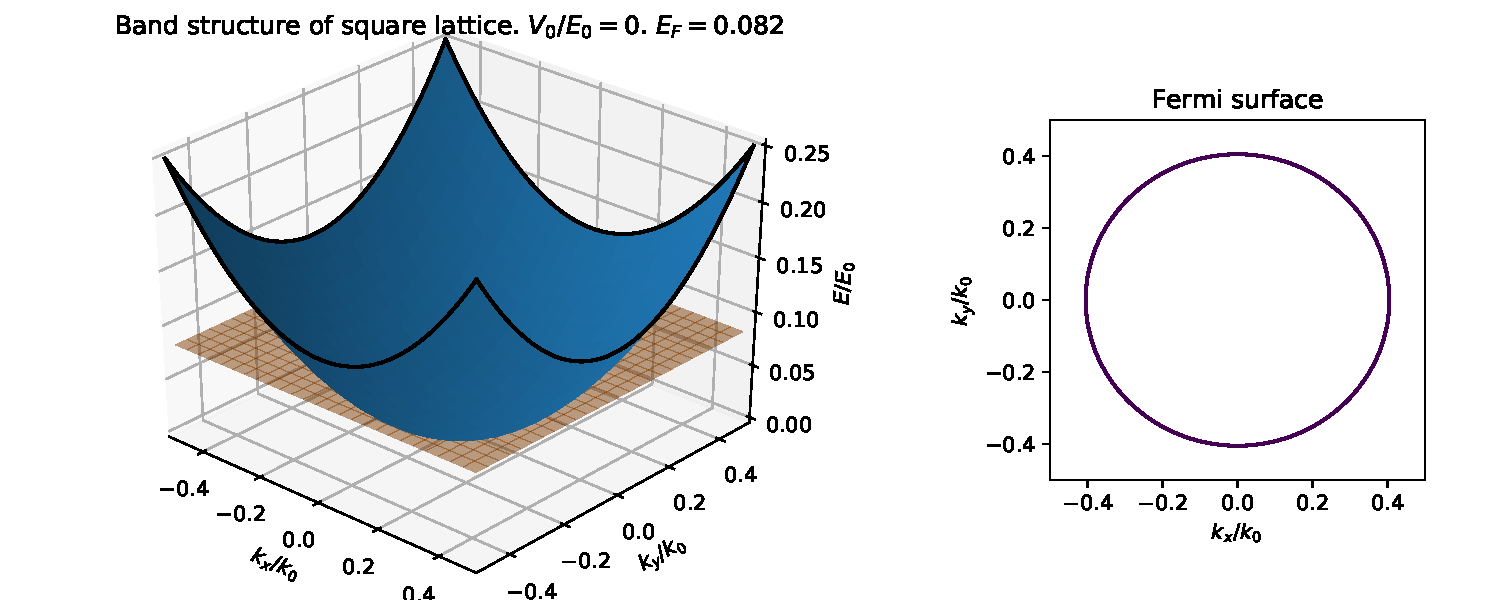
\includegraphics[width=\linewidth]{figures/band_structure_none.pdf}
		\caption{The dispersion relation for a free particle in a square lattice of monovalent atoms, along with the Fermi surface.}
		\label{fig:band_structure_none}
	\end{figure}

	\begin{figure}[h]
		\centering
		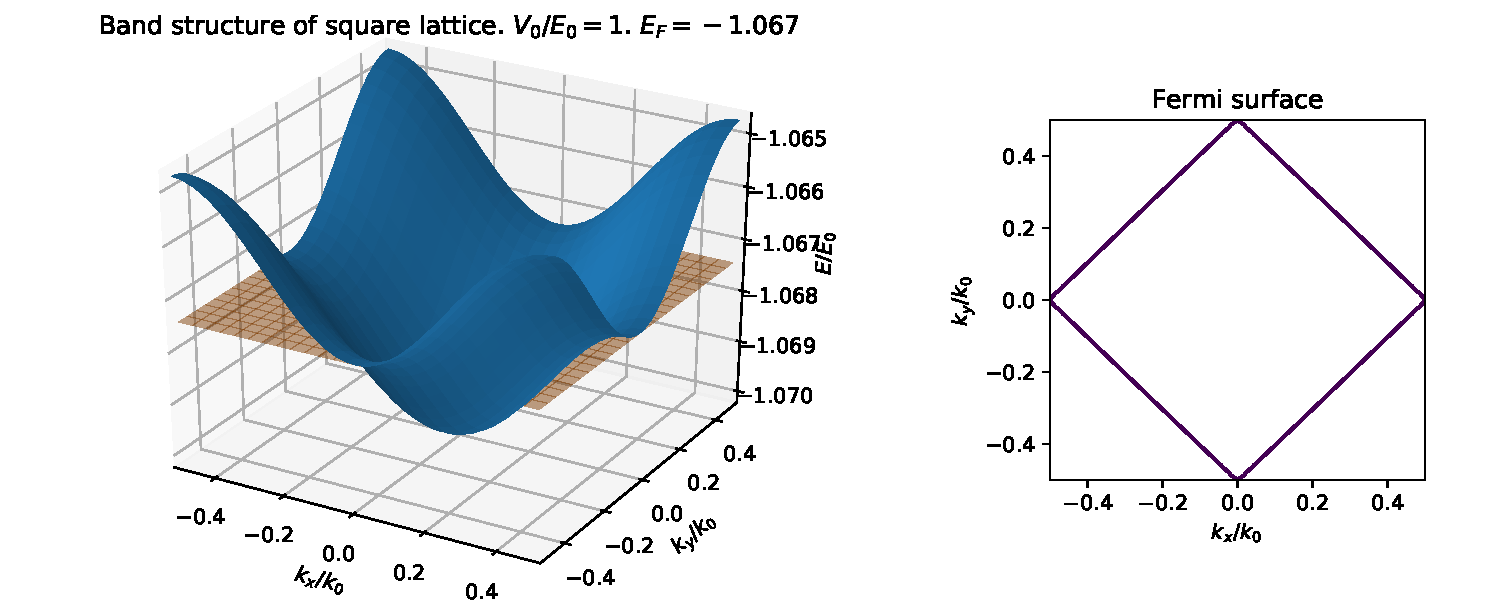
\includegraphics[width=\linewidth]{figures/band_structure_strong.pdf}
		\caption{The dispersion relation of a particle in a strong harmonic potential, on a square lattice of monovalent atoms, along with the corresponding Fermi surface.}
		\label{fig:band_structure_strong}
	\end{figure}

\end{document}